\chapter{Mathematical model}
In this chapter, we describe the basic relationships related to continuum dynamics relevant to this work. We will introduce equations describing flow in a free environment. We describe turbulent behavior and Reynolds decomposition. Furthermore, we will mention some characteristics important for describing blood flow in vessels. Finally, we summarize the assumptions further made on the mathematical model used in this work.

\section{Fluid Dynamics}
We will consider the fluid under study as a continuum, thus treating it as a perfectly continuous structure. The equations describing the dynamics of the continuum can be uniquely derived from the laws of conservation of mass, momentum, and energy. These equations are also linked with the physical properties of the studied environment and material.

In an isolated and isothermal system, the development of fluid dynamics over time can be expressed using a system of partial differential equations in the form
\\
\begin{subequations}\label{NS}
	\begin{gather}
		\label{a}
		\frac{\partial \rho}{\partial t} + \nabla \cdot (\rho \vec{u}) = 0, \\[5pt]
		\label{b}
		\frac{\partial (\rho \vec{u})}{\partial t} + \nabla \cdot (\rho \vec{u} \otimes \vec{u}) = \nabla \cdot \mathbf{T} + \rho \vec{g},
	\end{gather}
\end{subequations}
where the symbol $ \otimes $ denotes the outer product defined by components as $ (\vec{u} \otimes \vec{u})_{ij} = u_{i} u_{j}, \: i,j \in \{1,2,3\} $ \cite{Anderson}. The quantities in \eqref{NS} respectively represent
\begin{itemize}
	\item[]{\makebox[3cm]{$ \rho $ \si{[kg.m^{-3}]}\hfill} the density of the fluid,}
	\item[]{\makebox[3cm]{$ \vec{u} $ \si{[m.s^{-1}]}\hfill} the vector of macroscopic velocity,}
	\item[]{\makebox[3cm]{$ \mathbf{T} $ \si{[kg.m^{-1}.s^{-2}]}\hfill} the complete stress tensor,}
	\item[]{\makebox[3cm]{$ \vec{g} $ \si{[m.s^{-2}]}\hfill} the vector of acceleration of external forces.}
\end{itemize}
All quantities in \eqref{NS} are generally functions of time $ t $ \si{[s]} and position $ \vec{x} $~\si{[m]}.

The isothermal system can be supplemented with the equation of state of an ideal gas in the form
\begin{equation}\label{pressure}
	p = c^{2}_{s} \ \rho,
\end{equation}
where $ p $ \si{[Pa]} denotes pressure and $ c_{s} $ \si{[m.s^{-1}]} is the speed of sound in the fluid \cite{Latt}. In this case, \eqref{NS} together with \eqref{pressure} form a closed system that can be solved without the use of the law of conservation of energy.

\subsection{Stress Tensor and Force Effects}

We will denote the dynamic stress tensor as $\mathbf{T}_{\mu} = \big(\sigma^{\, \mu}_{ij} \,\big)$ \si{[kg.m^{-1}.s^{-2}]}, where $ i,j \in \{1,2,3\} $. For Newtonian fluids, the components of the dynamic stress tensor are linearly dependent on the spatial derivatives of velocity. Fluids that do not fulfill this linear dependence are called non-Newtonian. For the components of the dynamic stress tensor of Newtonian fluids, it holds that \cite{Schlichting}

\begin{subequations}\label{newton}
	\begin{eqnarray}
		\sigma^{\, \mu}_{ii} = \lambda \nabla \cdot \vec{u} + 2 \mu \frac{\partial u_i}{\partial x_i},&& \hspace{-3mm} i \in \{1,2,3\}, \\[5pt]
		\sigma^{\, \mu}_{ij} = \sigma^{\, \mu}_{ji} = \mu \ \left( \frac{\partial u_i}{\partial x_j} + \frac{\partial u_j}{\partial x_i} \right),&& \hspace{-4mm} \ i,j \in \{1,2,3\}, \: i \neq j,
	\end{eqnarray}
\end{subequations}
where $ \mu $ \si{[kg.m^{-1}.s^{-1}]} denotes the dynamic viscosity and $ \lambda $ \si{[kg.m^{-1}.s^{-1}]} is the so-called second viscosity coefficient~\cite{Cengel}. For Newtonian fluids, $\mathbf{T}_{\mu}$ is clearly a symmetric tensor. Further introducing the strain rate tensor~$\mathbf{D}~$ \si{[s^{-1}]} by the relation

\begin{equation}\label{eq:D}
	\mathbf{D} = \frac{1}{2} \left[ \nabla \vec{u} \ + \ (\nabla \vec{u})^T \right],
\end{equation}
the dynamic stress tensor can equivalently be rewritten in the form

\begin{equation}\label{eq:1}
	\mathbf{T}_{\mu} = 2 \mu \mathbf{D} \ + \ \left( \lambda + \frac{2}{3} \mu \right) \ (\nabla \cdot \vec{u}) \  \mathbf{I} \ ,
\end{equation}
where $ \mathbf{I} $ is the identity tensor of corresponding dimension. Using Stokes' hypothesis, $ \lambda = -\frac{2}{3} \mu $ \cite{Anderson}, which relates the dynamic viscosity and the second viscosity coefficient, the relation \eqref{eq:1} becomes

\begin{equation}
	\mathbf{T}_{\mu} = 2 \mu \mathbf{D}.
\end{equation}
Using $\mathbf{T}_{\mu}$, the complete stress tensor for a Newtonian fluid can further be written in the form
\begin{equation}\label{eq:T}
	\mathbf{T} = -p\mathbf{I} + \mathbf{T}_{\mu},
\end{equation}
where $ \mathbf{I} $ again is the identity tensor of corresponding dimension \cite{Cengel}.

The strain rate tensor is also used to define the shear rate $ \dot{\gamma} $~\si{[s^{-1}]} \cite{Cengel} by the relation
\begin{equation}\label{eq:dot gamma}
	\dot{\gamma} = \sqrt{2} \| \mathbf{D} \| _{F},
\end{equation}
where $ \| \cdot \| _{F} $ denotes the Frobenius matrix norm defined for a general matrix $ \mathbf{A} $ of dimensions $ m \times n $ with elements $ a_{ij} $ as
\begin{equation}
	\| \mathbf{A} \| _{F}  \coloneqq \sqrt{\sum_{i = 1}^{m} \sum_{j = 1}^{n} |a_{ij}|^2}.
\end{equation}

If the focus of investigation is the force effects of the fluid at the boundary of an object $ \partial \Omega $, we can express the components of the total force acting on $ \partial \Omega $ using \eqref{eq:T} as

\begin{equation}\label{eq:stress_int}
	{F}_{i} = \int\limits_{\partial\Omega}(\mathbf{T} \vec{n})_{i} \mathrm{d}S, \hspace{2mm} i \in \{1,2,3\},
\end{equation}
where $ \vec{n} $ denotes the normal vector to the boundary $ \partial \Omega $. The force expressed in this way represents the sum of the effects of pressure and viscous forces.

For describing the interaction of the fluid with an obstacle, the wall shear stress (in English \textit{wall shear stress}) \cite{WallStress} is often used, which we will denote by $ \tau _w $ \si{[kg.m^{-1}.s^{-2}]} and which is defined in 2D by the relation
\begin{equation}\label{eq:wall shear stress}
	\tau_w = \mathbf{T} \cdot \vec{t},
\end{equation}
where $ \vec{t} $ denotes the unit tangent vector at the wall at the point in question.

\subsection{Turbulence and Reynolds Decomposition}\label{turb}
We will refer to as turbulent any flow that is disordered in both time and space. The direction and magnitude of the velocity in turbulent flow constantly change, leading to generally irregular fluctuations. Turbulent flow exhibits a random and unstable character.

Turbulent flow can be observed at higher values of the Reynolds number, which is a dimensionless quantity defined as
\begin{equation}\label{Re}
	\mathrm{Re} = \dfrac{l_{0} u_{0}}{\nu} = \dfrac{l^{2}_{0}}{t_{0} \nu},
\end{equation}
where $ \nu $ is the kinematic viscosity \si{[m^2.s^{-1}]}, and $ l_{0} $~\si{[m]}, $ t_{0} $ \si{[s]}, and $ u_{0} $~\si{[m.s^{-1}]} are respectively the characteristic length, time, and velocity specific to the task at hand \cite{Landau}.

From the described properties of turbulent flow, it is clear that describing it is challenging. One approach to describing the turbulent flow field is through the statistical method of Reynolds' time averaging of quantities \cite{Sodja2007}, where a given quantity $ \psi $ is decomposed into its mean values $ \overline{\psi} $ and fluctuations $ \psi ' $ as
\begin{equation}
	\psi = \overline{\psi} + \psi '.
\end{equation}
The fluctuations $ \psi ' $ are defined such that the mean value $ \overline{\psi '} $ over a time period must be zero \cite{Schlichting}.

We emphasize that $ \psi $ in this case represents any scalar quantity, for which we may choose, for example, the components of velocity $ \vec{u}_i $, pressure $ p $, or density $ \rho $ \cite{Sodja2007}. Furthermore, it is important to note that the time interval for averaging
%, or control volume,
should be of an order of magnitude larger than the time
%, or spatial scale,
of the turbulent phenomena we wish to describe \cite{Sodja2007}.

If we now restrict ourselves to the Reynolds decomposition of the velocity field $ \vec{u} (\vec{x}, t) $ in terms of time averaging, we can introduce the turbulent kinetic energy $ T_{\text{turb}} $~\si{[m^{2}.s^{-2}]} by the relation
\begin{equation}\label{eq:turb kin energy}
	T_{\text{turb}} = \dfrac{1}{2} \left( \overline{(u_1 ')^2} + \overline{(u_2 ')^2} + \overline{(u_3 ')^2} \right) = \dfrac{1}{2} \left( \overline{(u_1 ')^2 + (u_2 ')^2 + (u_3 ')^2} \right),
\end{equation}
where we have used arithmetic rules when employing Reynolds decomposition \cite{Sodja2007}.

\section{Description of Vascular Flow}\label{cevni proudeni}
Due to the presence of numerous physical, chemical, and physiological processes, vascular flow represents a highly complex process. In many cases, however, a simplified model that neglects some characteristics suffices for its description \cite{Saloner2019}. In this section, we briefly describe some aspects for which a simplified model can be considered under appropriate assumptions.

\section*{\fontsize{11}{15}\selectfont Elasticity of Walls}
The interaction of an elastic body, i.e., a body with a movable boundary, can be modeled, for example, using the immersed boundary method \cite{Peskin}. In many cases, however, the elasticity of wall obstacles can be neglected, and only rigid geometry considered. Particularly in smaller vessels, neglecting the elasticity of the vascular walls has not shown a significant effect on the outcome. \cite{DempereMarco2006} However, this is not always the case, as significant non-negligible effects on the overall error of the results have been observed in the area of the aorta when considering rigid geometry. \cite{LANTZ2011}

Note that including the elasticity of vascular walls in the considered model requires appropriately defining the conditions of interaction with the fluid, which is generally a difficult task in vascular flow, often depending on the correct evaluation of \textit{in vivo} measurements. Additionally, in diseases such as arteriosclerosis\footnote{Arteriosclerosis is a disease in which the arterial walls thicken and subsequently lose their elasticity \cite{Fishbein2015}.}, vessels lose their elasticity in many patients, thus including elasticity in the model may not necessarily reflect the physiological state of the vessels correctly \cite{Saloner2019}.

\section*{\fontsize{11}{15}\selectfont Blood Viscosity}

For the mathematical model, it is important to choose the viscosity values correctly to encompass any non-Newtonian behavior of the fluid under investigation. Blood is generally considered a Newtonian fluid. However, there are situations where the Newtonian behavior of blood is compromised. For instance, in cases where the flow velocity of blood is very low, red blood cells can accumulate, consequently increasing the viscosity of blood.
Areas with such slow flow can be found, for example, in regions of aneurysmatic dilation\footnote{Aneurysmatic dilation refers to a disease condition where there is a local enlargement of a vessel \cite{Syed1997}.}. On the other hand, the viscosity of blood significantly decreases in areas where blood flows through very narrow vessels, particularly through vessels at the scale of arterioles or capillaries \cite{Saloner2019}.

There are viscosity models that aim to more accurately capture the physical description and behavior of blood viscosity~\cite{Saloner2019, Eichler2023, Boyd2007}. The simplest is the so-called Power-Law model \cite{Sequeira}. The Power-Law model prescribes for viscosity
\begin{equation}\label{eq:power-law}
	\mu _{\text{PL}} (\dot{\gamma}) = K_p  \dot{\gamma} ^{n_1-1} \ ,
\end{equation}
where $ K_p$ \si{[kg.m^{-1}]} and $ n_1 $ \si{[-]} are constants. Another model is the Casson model \cite{Boyd2007} which satisfies
\begin{equation}\label{eq:Casson}
	\mu _{\text{CA}} (\dot{\gamma}) = \frac{1}{\dot{\gamma}} \left[ k_{0} + k_{1} \sqrt{\dot{\gamma}} \right]^2 \ ,
\end{equation}
where $ k_1$ \si{[kg^{2}.m^{-2}]} and $ k_2 $ \si{[kg^{2}.m^{-2}]} are empirically determined constant parameters. A major advantage of these basic models is that for certain geometries and under specific conditions, exact solutions are available, which for example, provide reference values for numerical simulations. An obvious disadvantage of these models is their limited applicability, as they fail for shear rates approaching zero \cite{Boyd2007}.

Among the more complex models, the Cross model \cite{Sequeira} is defined by the relation
\begin{equation}\label{eq:cross}
	\mu _{\text{CR}} (\dot{\gamma}) = \frac{\mu_{0} - \mu_{\infty}}{1 + (k\dot{\gamma})^{n_2}} + \mu_{\infty}  \ ,
\end{equation}
where $ k $ \si{[s]} and $ n_2 $ \si{[-]} are constants, and it is also valid that
\begin{equation}\label{eq:m0 a minf}
	\mu _{0}  = \lim_{\dot{\gamma} \rightarrow 0+}\mu (\dot{\gamma})\, , \ \mu_{\infty} = \lim_{\dot{\gamma} \rightarrow \infty}\mu (\dot{\gamma}).
\end{equation}
The last mentioned model is the Carreau-Yasuda model \cite{Boyd2007} satisfying
\begin{equation}\label{eq:C-Y}
	\mu _{\text{CY}} (\dot{\gamma}) = \mu_{\infty} + (\mu_{0} - \mu_{\infty}) \left[ 1 + (\varepsilon \dot{\gamma}) ^{a} \right]^{\frac{n_3-1}{a}} \ ,
\end{equation}
where $ \varepsilon$ \si{[s]} , $a$ \si{[-]}, and $ n_3 $ \si{[-]} are again empirically determined constant parameters that influence the model behavior between boundary viscosity values. For $ \mu_{0}$ and $ \mu_{\infty} $ the condition \eqref{eq:m0 a minf} still applies.

All mentioned models are compared in Fig. \ref{fig:vs}, with parameter values taken from \cite{Eichler2023}.
\begin{figure}[H]
	\centering
	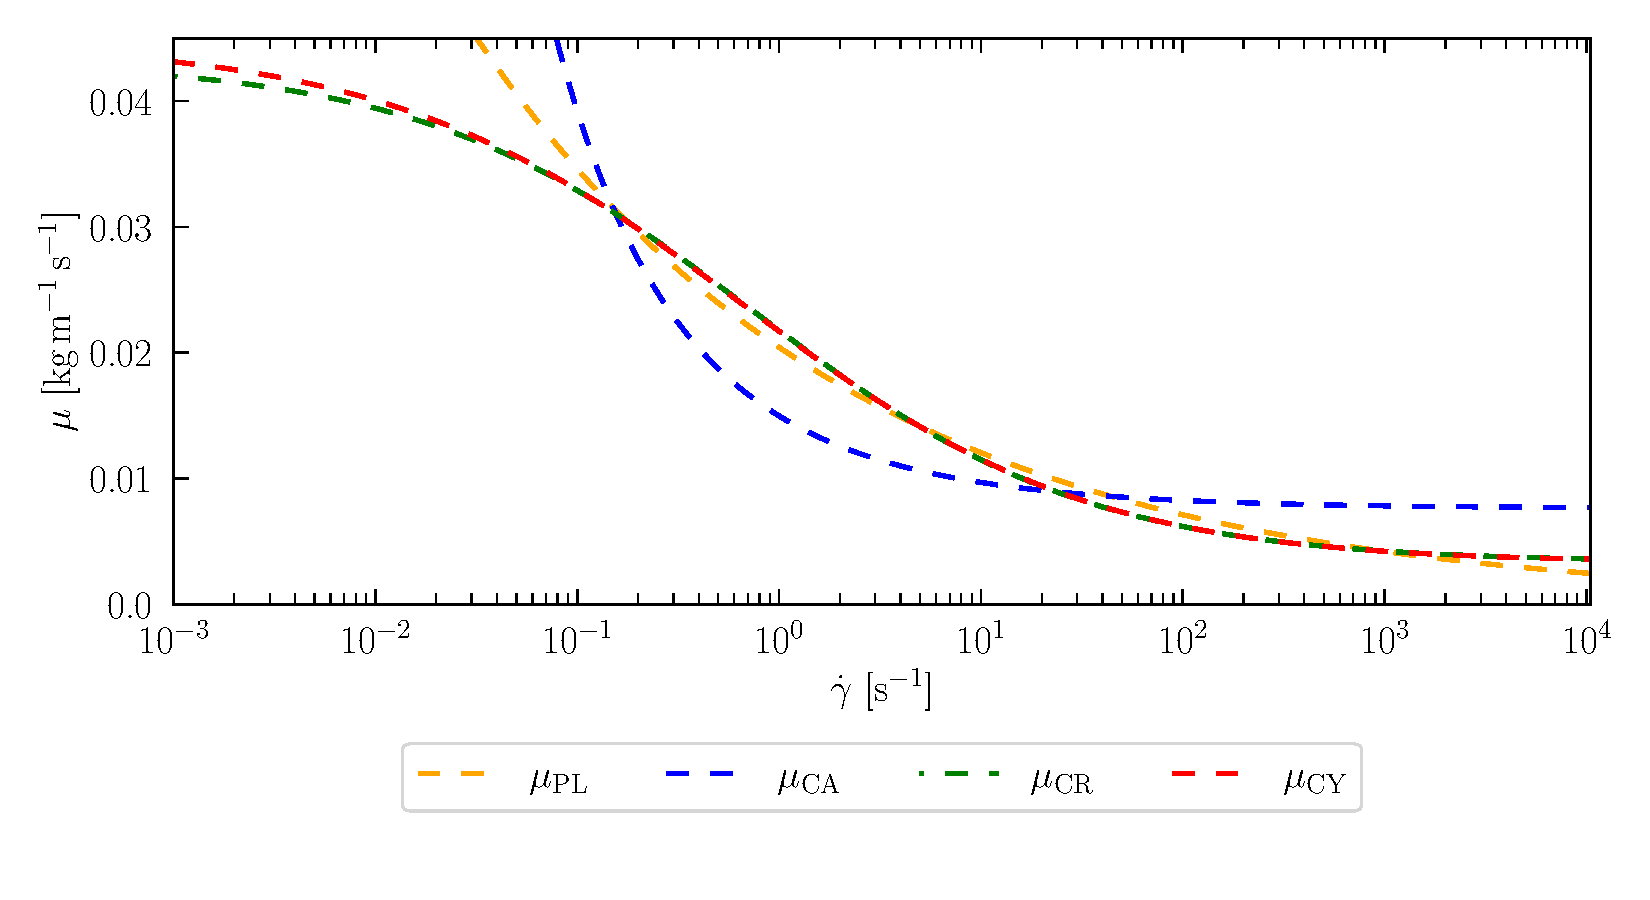
\includegraphics[width=1.0\textwidth]{figures/modely.pdf}
	\vspace{-9mm}
	\caption{Comparison of non-Newtonian viscosity models, specific parameter values were taken from \cite{Eichler2023}. Descriptions of each model correspond to the defining equations
		\eqref{eq:power-law}, \eqref{eq:Casson}, \eqref{eq:cross}, and \eqref{eq:C-Y}.}
	\label{fig:vs}
\end{figure}
We note that in this work, blood will be considered exclusively as a Newtonian fluid.

\section*{\fontsize{11}{15}\selectfont Turbulent Flow}
In most cases, blood flow can be approximated by laminar flow \cite{Sequeira}. However, in some instances in vascular flow, turbulence and chaotic behavior occur \cite{Saqr2020}. One area where turbulence can be observed is behind a vascular stenosis\footnote{Vascular stenosis is a condition in which there is a local narrowing of a vessel \cite{Carabello2009}.} \cite{Jain2022}. The flow velocity of blood in the narrowed area can significantly increase, and the reduction in the diameter of the vessel ensures that the flow remains laminar in this section of the constriction \cite{Sequeira}. However, immediately after the constriction, the flow velocity remains elevated even in areas with the original diameter, which can lead to the formation of vortices and a change in flow regime \cite{Saloner2019, Varghese2003}.

The occurrence of turbulent flow is physiologically undesirable as it is often accompanied by significant dissipation of kinetic energy, which can strain parts of the circulatory system. Additionally, vascular areas with turbulence show increased strain on vessel walls, which can lead to tissue damage and diseases such as arteriosclerosis. Therefore, it is desirable to minimize turbulence in blood flow \cite{Saloner2019, Kameneva2004}.

\section{Assumptions of the Mathematical Model in This Work}\label{pred}
Finally, we summarize the additional assumptions we will consider in our system. These assumptions simplify the solution of the system \eqref{NS}. Specifically, in this work, we will consider only an isothermal system (i.e., its temperature is constant over time), on which no external forces act. The considered fluid is also incompressible, Newtonian, and with constant dynamic viscosity.

We will consider a rectangular area $ \Omega \subset \mathbb{R}^2 $, $ \Omega = (0, L_1) \times (0, L_2) $, where $ L_1, L_2 $ \si{[m]} are the dimensions of the rectangle, and the time interval $ \mathcal{I} = \langle 0, T \rangle,$ where $ T > 0$. Let's denote

The equations \eqref{NS} solved on $ \Omega \times \mathcal{I} $ with these assumptions reduce to \cite{Schlichting}

\begin{subequations}\label{NS s predpoklady}
	\begin{gather}
		\label{a s predpoklady}
		\nabla \cdot \vec{u} = 0, \\[5pt]
		\label{b s predpoklady}
		\rho \frac{\text{D} \vec{u}}{\text{D} t} = - \nabla p + \mu \Delta \vec{u},
	\end{gather}
\end{subequations}
where we used the notation of the material derivative operator
\begin{equation}
	\dfrac{\text{D}}{\text{D} t} \coloneqq \dfrac{\partial}{\partial t} + \vec{u} \cdot \nabla.
\end{equation}

We denote $ \partial \Omega_{\text{in}} $ as the part of the boundary of the area $ \Omega $ where the boundary condition at the inlet is prescribed, $ \partial \Omega_{\text{out}} $ as the part of the boundary where the boundary condition at the outlet is prescribed, and $ \partial \Omega_{\text{w}} $ as the part of the boundary where the interface between the fluid and the solid exists and where a no-slip boundary condition is considered. Then the equations \eqref{NS s predpoklady} are supplemented by initial and boundary conditions
\begin{subequations}\label{eq:okrajovky}
	\begin{alignat}{3}
		&\vec{u} = \vec{u}_{\text{ini}},  &p = p_{\text{ini}} \hspace{5mm} &\text{on } \ \Omega \times \mathcal{I}\\[3pt]
		&(\nabla p - \nu \Delta \vec{u}) \cdot \vec{n}  = 0, &\vec{u} = \vec{u}_{\text{in}} \hspace{5mm} &\text{on } \ \partial \Omega_{\text{in}} \times \mathcal{I}\\[3pt]
		&\vec{u} = \vec{0}, \, &\nabla p \cdot \vec{n} = 0 \hspace{5mm} &\text{on } \ \partial \Omega_{\text{w}} \times \mathcal{I}\\[3pt]
		&p = p_{\text{out}}, &\nabla u_i \cdot \vec{n} = 0 \hspace{5mm} &\text{on } \ \partial \Omega_{\text{out}} \times \mathcal{I}, \, i = 1, 2 \ ,
	\end{alignat}
\end{subequations}
where $ \vec{n} $ is the unit external normal vector to the boundary of the considered area, $ \vec{u}_{\text{ini}}$ \si{[m.s^{-1}]} or $ p_{\text{ini}} $ \si{[kg.m^{-1}.s^{-2}]} is the initial velocity or initial pressure, respectively, $ \vec{u}_{\text{in}}$ \si{[m.s^{-1}]} is the velocity prescribed at the inlet, and $ p_{\text{out}} $~\si{[kg.m^{-1}.s^{-2}]} is the pressure prescribed at the outlet. Initial and boundary conditions are further discussed in section~\ref{pocatecni a okrajove podminky}.
